 


\newcommand{\defi}[1]{\emph{#1}}                 %



\newcommand{\spacefont}{\mathcal}                %

\newcommand{\signper}[1]{\({#1}\sig\)-oriented}  %


\newcommand{\lrar}{\longrightarrow}
\newcommand{\lto}{\longrightarrow}
\newcommand{\llar}{\longleftarrow}
\newcommand{\hrar}{\hookrightarrow}
\newcommand{\hlar}{\hookleftarrow}
\newcommand{\wtl}{\widetilde}
\newcommand{\what}{\widehat}
\newcommand{\st}{\stackrel}
\newcommand{\ovl}{\overline}
\newcommand{\ol}{\overline} %


\newcommand{\adj}{\mathbin{%
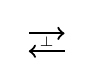
\begin{tikzpicture}[baseline,thick] 
\coordinate (source) at (0ex,.5ex);
\coordinate (target) at (3ex,.5ex);
\draw[->] ([yshift=1ex]source) -- ([yshift=1ex]target); 
\draw[->] ([yshift=-.5ex]target) -- ([yshift=-.5ex]source);
\node at (1.5ex,.8ex) {$\scriptscriptstyle \perp$};
\end{tikzpicture}%
}}

\newcommand{\locadj}{\mathbin{%
    \begin{tikzpicture}[baseline=-0.8ex]
	\coordinate (source) at (0ex,0ex);
	\coordinate (target) at (3ex,0ex);
	\draw[-stealth] ([yshift=0.7ex]source) to ([yshift=0.7ex]target);
    \draw[left hook-stealth] ([yshift=-0.85 ex]target) to ([yshift=-0.85 ex]source);
	\node at (1.5ex,0  ex) {$\scriptscriptstyle \perp$};
    \end{tikzpicture}
}}


\newcommand{\locadjL}[1]{\mathbin{%
    \begin{tikzpicture}[baseline=-0.8ex]
	\coordinate (source) at (0ex,0ex);
	\coordinate (target) at (3ex,0ex);
	\draw[-stealth] ([yshift=0.7ex]source) to node[above]{\scriptsize $#1$}([yshift=0.7ex]target);
    \draw[left hook-stealth] ([yshift=-0.85 ex]target) to ([yshift=-0.85 ex]source);
	\node at (1.5ex,0  ex) {$\scriptscriptstyle \perp$};
    \end{tikzpicture}
}}


\newcommand{\bigcircle}{\bigcirc}  %


\newcommand{\oneover}[1]{{\scriptstyle \frac{1}{#1}}}   %
\newcommand{\onehalf}{\oneover{2}}   %
\newcommand{\oneoverl}{\oneover{l}}   %
\newcommand{\comma}{,}                     %


\newcommand{\myperp}{\scalebox{0.5}{\rotatebox{270}{$\dashv$}}} %

\newcommand{\cocolon}{\nobreak \mskip6mu plus1mu \mathpunct{}\nonscript\mkern-\thinmuskip {:}\mskip2mu \relax}

\makeatletter
\newcommand{\dovl}[1]{\overline{\dbl@overline{#1}}}
\newcommand{\dbl@overline}[1]{\mathpalette\dbl@@overline{#1}}
\newcommand{\dbl@@overline}[2]{%
  \begingroup
  \sbox\z@{$\m@th#1\overline{#2}$}%
  \ht\z@=\dimexpr\ht\z@-2\dbl@adjust{#1}\relax
  \box\z@
  \ifx#1\scriptstyle\kern-\scriptspace\else
  \ifx#1\scriptscriptstyle\kern-\scriptspace\fi\fi
  \endgroup
}
\newcommand{\dbl@adjust}[1]{%
  \fontdimen8
  \ifx#1\displaystyle\textfont\else
  \ifx#1\textstyle\textfont\else
  \ifx#1\scriptstyle\scriptfont\else
  \scriptscriptfont\fi\fi\fi 3
}
\makeatother



\newcommand{\alp}{\alpha}
\newcommand{\bet}{\beta}
\newcommand{\gam}{\gamma}
\newcommand{\Del}{\Delta}
\newcommand{\del}{\delta}
\newcommand{\Lam}{\Lambda}
\newcommand{\Om}{\Omega}
\newcommand{\om}{\omega}
\newcommand{\Sig}{\Sigma}
\newcommand{\sig}{\sigma}
\newcommand{\vphi}{\varphi}
\newcommand{\eps}{\epsilon}

\newcommand{\cT}{\mathcal{T}} 





\newcommand{\NN}{\mathbb{N}}               %
\newcommand{\RR}{\mathbb{R}}               %
\newcommand{\CC}{\mathbb{C}}               %
\newcommand{\ZZ}{\mathbb{Z}}               %
\newcommand{\QQ}{\mathbb{Q}}               %
\newcommand{\FF}{\mathbb{F}}               %

\newcommand{\nO}{\mathcal{O}}               %

\newcommand{\im}{\mathrm{im}}              %
\newcommand{\coker}{\mathrm{coker}}        %
\newcommand{\Tor}{\mathrm{Tor}}            %

\newcommand{\Mat}{\mathrm{Mat}}            %

\newcommand{\odd}{\mathrm{odd}}            %

\newcommand{\spec}{\mathrm{spec}}          %

\newcommand{\fp}{\mathfrak{p}}             %
\newcommand{\fb}{\mathfrak{b}}             %

\newcommand{\Div}{\mathrm{Div}}            %
\newcommand{\val}{\mathrm{val}}            %

\newcommand{\cd}{\mathrm{cd}}              %
\newcommand{\vcd}{\mathrm{vcd}}            %


\newcommand{\pt}{\mathrm{pt}}                    %

\newcommand{\Hom}{\operatorname{Hom}}            %
\newcommand{\End}{\operatorname{End}}            %
\newcommand{\Aut}{\operatorname{Aut}}            %


\newcommand{\fib}{\operatorname{fib}}            %
\newcommand{\hofib}{\operatorname{hofib}}        %
\newcommand{\cof}{\operatorname{cof}}            %
\newcommand{\coeq}{\operatorname{coeq}}		 %

\newcommand{\colim}{\mathop{\mathrm{colim}}}     %
\newcommand{\hocolim}{\mathop{\mathrm{hocolim}}} %
\newcommand{\TotCof}{\mathrm{TotCof}}		 %

\newcommand{\Map}{\operatorname{Map}}            %

\newcommand{\grpcr}{\iota}                       %
\newcommand{\core}{\mathrm{Cr}}                  %
\newcommand{\Core}{\core}                        %

\newcommand{\cor}{\mathrm{Cor}}                  %

\newcommand{\Dec}{\mathrm{dec}}                  %
\newcommand{\dec}{\mathrm{dec}}                  %

\newcommand{\lag}{\operatorname{lag}}            %

\newcommand{\idem}{\mathrm{idem}}                %
                                                 %
\newcommand{\mn}{\mathrm{min}}                  %


\newcommand{\nerv}{\operatorname N}              %
\newcommand{\Ho}{\operatorname{Ho}}              %

\newcommand{\LKan}{\operatorname{Lan}}           %

\newcommand{\Pro}{\operatorname{Pro}}            %
\newcommand{\Ind}{\operatorname{Ind}}            %
\newcommand{\Tate}{\operatorname{Tate}}          %
\newcommand{\Latt}{\operatorname{Latt}}          %


\newcommand{\coev}{\mathrm{coev}}                %

\newcommand{\op}{^\mathrm{op}}                   %
\newcommand{\mop}{\mathrm{op}}                   %

\newcommand{\Ar}{\operatorname{Ar}}              %
\newcommand{\Artex}{\operatorname{Ar^{\mathrm{tex}}}} %
\newcommand{\Twar}{\operatorname{TwAr}^{\mathrm{r}}}          %
\newcommand{\XYZ}{\mathrm{DoAr}}                 %

\newcommand{\dom}{\mathrm{dom}}                  %
\newcommand{\cod}{\mathrm{cod}}                  %
\newcommand{\target}{\mathrm{t}}                 %
\newcommand{\source}{\mathrm{s}}                 %

\newcommand{\ran}{\mathrm{ran}}                  %

\newcommand{\cp}{\omega}                         %
\newcommand{\perf}{\mathrm{p}}                   %


\newcommand{\Barc}{\operatorname{B}}             %
\newcommand{\Mon}{\operatorname{Mon}}            %
\newcommand{\Grp}{\operatorname{Grp}}            %
\newcommand{\grp}{\mathrm{grp}}                  %

\newcommand{\Bs}{\mathrm{B}}                     %

\newcommand{\sd}{\operatorname{sd}}              %

\newcommand{\gr}[1]{|#1|}                        %

\newcommand{\asscat}{\operatorname{asscat}}      %
\newcommand{\snerv}{\operatorname{N}}            %
\newcommand{\comp}{\operatorname{comp}}	         %


\newcommand{\rF}{\mathrm{F}}   %
\newcommand{\rU}{\mathrm{U}}   %

\newcommand{\pr}{\mathrm{pr}}                %
\newcommand{\inc}{\mathrm{inc}}              %
\newcommand{\incl}{\mathrm{inc}}             %
                                             %
\newcommand{\id}{\mathrm{id}}                %
\newcommand{\const}{\mathrm{const}}          %

\newcommand{\Spa}{{\mathcal Sp}}             %
\newcommand{\Spaf}{\Spa^{\free}}             %
\newcommand{\Spap}{\Spa^{\cp}}               %
\newcommand{\PSp}{{\mathcal {PS}p}}          %
\newcommand{\Sps}{\mathcal S}                %
\newcommand{\bigSps}{\textsc{S}}	     %
\newcommand{\Sfinast}{{\mathcal S^\mathrm{fin}_*}}%
\newcommand{\Sfin}{{\mathcal S^\mathrm{fin}}}  %


\newcommand{\swedge}{\times}                   %
\newcommand{\cwedge}{{\scriptscriptstyle\wedge}} %
\newcommand{\ssmash}{\otimes}                  %
\renewcommand{\hom}{\operatorname{hom}}        %
\newcommand{\map}{\operatorname{hom}}          %

\newcommand{\barsm}{\boxtimes}		       %

\newcommand{\Ominfty}{\Omega^{\infty}}         %

\renewcommand{\SS}{\mathbb{S}}                 %

\newcommand{\sph}{\mathrm{S}}                  %

\newcommand{\solid}{localisation\xspace}       %
\newcommand{\compatible}{compatible\xspace}    %


\newcommand{\h}{\mathrm{h}}                    %
\newcommand{\Ct}{\mathrm{C_2}}                 %
\newcommand{\BC}{\Bs \Ct}                      %
\newcommand{\hC}{{\h\Ct}}                      %
\newcommand{\tC}{{\mathrm{t}\Ct}}              %
\newcommand{\undl}{\mathrm{u}}                 %
\newcommand{\geofix}{{\varphi\Ct}}             %
\newcommand{\geoFix}{{\Phi^\Ct}}               %
\newcommand{\gC}{{\mathrm{g}\Ct}}              %
\newcommand{\Spagc}{\Spa^\gC}                  %
\newcommand{\gCt}{\gC}                         %

\newcommand{\Th}{\mathrm{Th}}		       %

\newcommand{\TDelta}{\Delta}                   %
                                               %
\newcommand{\N}{\mathrm{N}}                    %
\newcommand{\Ne}{\mathrm{N}}                   %
\newcommand{\Norm}{\mathrm{N}}                 %
\newcommand{\taut}{\mathrm t}                  %

\newcommand{\tran}{\mathrm tran}     %
\newcommand{\res}{\mathrm res}      %


\newcommand{\Aeff}{\mathrm{A^{\hspace{-.2ex}eff}}} %
\newcommand{\uAeff}{\underline{\Aeff}}         %

\newcommand{\OCt}{\mathbf{O}_{\Ct}}                        %
\newcommand{\uCatp}{\underline{\mathrm{Cat}}^\mathrm{p}_\infty}
\newcommand{\uCath}{\underline{\mathrm{Cat}}^\mathrm{h}_\infty}
\newcommand{\uFunq}{\underline{\mathrm{Fun}}^\mathrm{q}_\infty}




\newcommand{\Ab}{\mathcal{A}b}                   %
\newcommand{\Mack}{\mathcal{M}a_{\Ct}}                   %

\newcommand{\Vect}{\mathrm{Vect}}                %
\newcommand{\chr}{\mathrm{char}}                 %

\newcommand{\CMonoids}{\mathrm{CMon}}            %
\newcommand{\CMon}{\CMonoids}                    %

\newcommand{\one}{\mathbf{1}} 			 %

\newcommand{\Ring}{\mathrm{Ring}}                %

\newcommand{\Mod}{\operatorname{Mod}}            %
\newcommand{\lin}{\mathrm{lin}}                  %
\newcommand{\LMod}{\mathrm{LMod}}                %

\newcommand{\fg}{{\mathrm{f}}}                   %

\newcommand{\Proj}{\mathrm{Proj}}                %
\newcommand{\Prof}[1]{\Proj(#1)}                 %
\newcommand{\Free}{\mathrm{Free}}                %

\newcommand{\Modcp}{\Mod^{\cp}}                  %

\newcommand{\Modp}[1]{\Modcp({#1})}              %
\newcommand{\Modf}[1]{\mathrm{Mod}^\fg({#1})}    %
\newcommand{\Modc}[2]{\mathrm{Mod}^{#1}({#2})}   %

\newcommand{\Torf}{\mathrm{Tor}^{\mathrm{f}}}    %

\newcommand{\gl}{\mathrm{gl}}                    %
\newcommand{\Unimod}{\mathrm{Unimod}}            %

\newcommand{\Ering}{\mathrm{E}}			 %
\newcommand{\Ek}[1]{{\Ering_{#1}}}               %
\newcommand{\Einf}{\Ek{\infty}}          	 %
\newcommand{\Eone}{\Ek{1}}               	 %

\newcommand{\Alg}{\mathrm{Alg}}                  %
\newcommand{\Sq}{\mathrm{Sq}}			%


\newcommand{\Ch}{\operatorname{Ch^b}}            %

\newcommand{\CHom}{\underline{\Hom}}	         %
\newcommand{\HHom}{\operatorname{Hom}^{\mathrm{cx}}} %
\newcommand{\DHom}{\mathcal{H}om}                %
\newcommand{\qiso}{\mathrm{qIso}}                %
\newcommand{\iso}{\mathrm{Iso}}                  %

\newcommand{\GEM}{\mathrm{H}}                    %

\newcommand{\Cone}{\operatorname{Cone}}          %

\newcommand{\Der}{\mathcal D}                    %
\newcommand{\Dfree}{{\mathcal D}^\fg}            %
\newcommand{\Dperf}{{\mathcal D}^\perf}          %
\newcommand{\Perf}{\Dperf}                       %

\newcommand{\free}{\mathrm{f}}                   %

\newcommand{\Psh}{\operatorname{Psh}}            %
\newcommand{\PSh}{\Psh}                          %

\newcommand{\dg}{\mathrm{dg}}                    %

\newcommand{\rH}{\mathrm{H}}                     %

\newcommand{\Fr}{\mathrm{Fr}}                    %


\newcommand{\Com}{\mathrm{Com}}       %
\newcommand{\Day}{\mathrm{Day}}       %
\newcommand{\Sm}{\mathrm{Sm}}			%
\newcommand{\MCom}{\mathrm{MCom}}     %
\newcommand{\CAlg}{\mathrm{CAlg}}     %
\newcommand{\Op}{\mathrm{Op}_\infty}  %

\newcommand{\Mul}{\mathrm{Mul}}       %

\newcommand{\Fin}{\mathrm{Fin}}       %
\newcommand{\<}{\langle}			%
\renewcommand{\>}{\rangle}			%

\newcommand{\act}{\mathrm{act}}			%
\newcommand{\mon}{\mathrm{mon}}			%



\newcommand{\et}{\text{ét}}                      %


\newcommand{\Posets}{\text{Posets}}             %
\newcommand{\Set}{\mathrm{Set}}                  %
\newcommand{\Top}{\mathrm{Top}}                 %

\newcommand{\Cat}{\mathrm{Cat}_\infty}                  %
\newcommand{\Catfin}{\mathrm{Cat}_{\infty,\mathrm{fin}}}%
\newcommand{\CAT}{\mathrm{CAT}_\infty}                  %
\newcommand{\CATast}{\mathrm{CAT}_{\infty,\ast}}                   %
\newcommand{\CATust}{\CAT^\ast}                   %
\newcommand{\PrL}{\mathrm{Pr}^{\mathrm{L}}}  %
\newcommand{\PrR}{\mathrm{Pr}^{\mathrm R}}
\newcommand{\Catx}{\Cat^\ex}     %
\newcommand{\Catxast}{\mathrm{Cat}^\ex_{\infty,\ast}}                %
\newcommand{\Catxom}{\Cat^\mathrm{ex,\perf}}    %
\newcommand{\Catxi}{\mathrm{Cat}^{\ex,\natural}_{\infty}}                 %
\newcommand{\Catxmn}{\mathrm{Cat}^\ex_{\infty,\mn}}                   %
\newcommand{\CatxK}{\Catx[\mathrm{Kar}^{-1}]}    %

\newcommand{\sCatx}{\mathrm{s}\Catx}             %
\newcommand{\Catrex}{\mathrm{Cat}_\infty^\mathrm{rex}}   %

\newcommand{\sSps}{\mathrm{s}\Sps}	 %
\newcommand{\cSS}{\mathrm{cS}\Sps}	         %

\newcommand{\CatSpa}{\mathrm{Cat}_{\Spa}}               %
\newcommand{\CatSpaPt}{\mathrm{Cat}_{\Spa,\ast}}               %
\newcommand{\CatxSpaPt}{(\Catx)_{\Spa,\ast}}               %


\newcommand{\Cath}{\mathrm{Cat}^\mathrm{h}_\infty}      %
\newcommand{\sCath}{\mathrm{s}\Cath} 	                %
\newcommand{\Catnh}{\mathrm{Cat}^\mathrm{nh}_\infty}    %
\newcommand{\Catsb}{\mathrm{Cat}^\mathrm{sb}_\infty}    %
\newcommand{\Catps}{\mathrm{Cat}^\mathrm{ps}_\infty}    %
\newcommand{\Catp}{\mathrm{Cat}^{\mathrm p}_\infty}     %
\newcommand{\Catpkappa}{\mathrm{Cat}^{\mathrm p}_{\infty,\kappa}}          %
\newcommand{\Catpi}{\mathrm{Cat}^{\mathrm p,\natural}_{\infty}}                 %
\newcommand{\Cathi}{\mathrm{Cat}^{\mathrm h,\natural}_{\infty}}       
\newcommand{\Catd}{\mathrm{Ring}^{\mathrm p}}         %

\newcommand{\sCatp}{\mathrm{s}\Catp}             %


\newcommand{\Bord}{\operatorname{Bord}}          %
\newcommand{\Span}{\operatorname{Span}}          %
\newcommand{\coSpan}{\operatorname{coSpan}}      %
\newcommand{\Hlgy}{\operatorname{Hlgy}}          %
\newcommand{\Cob}{\mathrm{Cob}}                  %
\newcommand{\Cobdelta}{{\mathrm{Cob}^\partial}}  %
\newcommand{\Seq}{\operatorname{Seq}}            %
\newcommand{\seq}{\mathrm{seq}}                  %


\newcommand{\Fun}{\operatorname{Fun}}            %
\newcommand{\Nat}{\operatorname{Nat}}            %
\newcommand{\nat}{\operatorname{nat}}            %
\newcommand{\fun}{\overline{\operatorname{Fun}}^{\hspace{0.1em}\ex}}  %

\newcommand{\sm}{\mathrm{sm}}			 %

\newcommand{\ex}{\mathrm{ex}}                    %
\newcommand{\lex}{\mathrm{lex}}                  %
\newcommand{\rex}{\mathrm{rex}}                  %
\newcommand{\coh}{\mathrm{coh}}                  %

\newcommand{\FunR}{\operatorname{Fun^R}}         %
\newcommand{\FunL}{\operatorname{Fun^L}}         %

\newcommand{\sifted}{\mathrm{sif}}               %
\newcommand{\filt}{\mathrm{filt}}                %
\newcommand{\fin}{\mathrm{fin}}                  %
\newcommand{\Funfin}{\Fun^{\fin}}                %
\newcommand{\Funrex}{\Fun^{\rex}}		 %
\newcommand{\diag}{\Del}                         %

\newcommand{\BiFun}{\operatorname{BiFun}}        %
\newcommand{\red}{\mathrm{red}}                  %
\newcommand{\Funr}{{\Fun_*}}                     %
\newcommand{\Funexc}{\Fun^{2-\mathrm{exc}}}      %
\newcommand{\Excr}{{\operatorname{Exc}_*}}       %
\newcommand{\Funexcr}{\Fun^{2-\mathrm{exc}}_*}   %
\newcommand{\Funpoly}{\Fun^{2-\mathrm{poly}}_*}  %
\newcommand{\App}{\mathrm{P}}                    %
\newcommand{\rT}{\mathrm{T}}                     %
\newcommand{\BiFib}{\mathrm{BiFib}}              %
\newcommand{\RFib}{\operatorname{RFib}}          %
\newcommand{\LaxAr}{\mathrm{LaxAr}}             %


\newcommand{\add}{\mathrm{add}}                  %
\newcommand{\vloc}{\mathrm{vloc}}                %
\newcommand{\kloc}{\mathrm{kloc}}                %
\newcommand{\brd}{\bord}                %
\newcommand{\binv}{\mathrm{binv}}

\newcommand{\Funadd}{\Fun^\add}                  %
\newcommand{\Funaddbord}{\Fun^{\add-\brd}}                  %

\newcommand{\Funvloc}{\Fun^\vloc}                  %
\newcommand{\Funkloc}{\Fun^\kloc}                  %
\newcommand{\Funbord}{\Fun^\brd}                  %
\newcommand{\Funaddfilt}{\Fun^{\add,\filt}}       %
\newcommand{\Funklocfilt}{\Fun^{\kloc,\filt}}      %

\newcommand{\Funaddk}[1][\filt]{\Fun^{\add}_{#1}}     %
\newcommand{\Funklock}[1][\filt]{\Fun^{\kloc}_{#1}}   %
\newcommand{\Funklocbordk}[1][\filt]{\Fun^{\kloc-\brd}_{#1}}   %

\newcommand{\Funaddbordk}[1][\filt]{\Fun^{\add-\brd}_{#1}}
\newcommand{\Funk}[1][\filt]{\Fun_{#1}}
\newcommand{\Funbordk}[1][\filt]{\Fun^{\brd}_{#1}}

\newcommand{\Funklocbord}{\Fun^{\kloc-\brd}}                  %



\newcommand{\dM}{\mathcal{M}}                    %


\newcommand{\Funx}{\operatorname{Fun^{ex}}}      %
\newcommand{\Funq}{\operatorname{Fun^q}}         %
\newcommand{\Funqhom}{\operatorname{Fun^{hom}}}  %
\newcommand{\Funqcoh}{\operatorname{Fun^{coh}}}  %
\newcommand{\Funnq}{\operatorname{Fun^{nq}}}     %
\newcommand{\Funpq}{\operatorname{Fun^{p}}}      %
\newcommand{\Funs}{\operatorname{Fun^s}}         %
\newcommand{\Funb}{\operatorname{Fun^b}}         %
\newcommand{\Funpb}{\operatorname{Fun^{pb}}}	 %
\newcommand{\Funnb}{\operatorname{Fun^{nb}}}    %
\newcommand{\Funh}{\operatorname{Fun^h}}         %
\newcommand{\Funp}{\operatorname{Fun^p}}         %
\newcommand{\Funns}{\operatorname{Fun^{ns}}}     %
\newcommand{\Funps}{\operatorname{Fun^{ps}}}     %

\newcommand{\Null}{\operatorname{Null}}          %
\newcommand{\Pairings}{\operatorname{Pair}}      %
                                                 %
\newcommand{\pair}{\mathrm{pair}}                %

\newcommand{\Catb}{\mathrm{Cat}^\mathrm{b}_\infty}             %
\newcommand{\Catpb}{\mathrm{Cat}^\mathrm{pb}_\infty}           %
\newcommand{\BiFibp}{\mathrm{BiFib^{p}}}         %


\newcommand{\metstab}{\mathrm{stab}}             %
\newcommand{\ads}{\mathrm{ad}}                   %


\newcommand{\Catpom}{\mathrm{Cat^{p,\cp}}}       %
\newcommand{\Catpcp}[1][\cp]{\mathrm{Cat^{p}_{#1}}}%
\newcommand{\Catcp}[1][\cp]{\mathrm{Cat^{ex}_{#1}}}%

\newcommand{\Motp}[1][]{{\if\relax\detokenize{#1}\mathrm{Mot^p}\relax\else\mathrm{Mot}_{#1}^{\mathrm{p}}\fi}}  %
\newcommand{\Motpun}[1][]{\mathrm{Mot^p_{un\if\relax\detokenize{#1}\relax\else{,}#1\fi}}}           %
\newcommand{\Motpom}{\mathrm{Mot^{p,\cp}}}       %
\newcommand{\Motploc}{\mathrm{LMot^p}}           %
\newcommand{\Motkar}[1][]{{\if\relax\detokenize{#1}\mathrm{Mot^{k}}\relax\else\mathrm{Mot^k_{#1}}\fi}}  %
\newcommand{\Motpbordun}{\mathrm{BMot^p_{un}}}   %
\newcommand{\Motpomun}{\mathrm{Mot^{p,\cp}}_{un}}%
\newcommand{\Motpbord}[1][]{{\if\relax\detokenize{#1}\mathrm{Mot^{pw}}\relax\else\mathrm{Mot}_{#1}^{\mathrm{pw}}\fi}} %
\newcommand{\Mot}[1][]{{\if\relax\detokenize{#1}\mathrm{Mot}\relax\else\mathrm{Mot_{#1}}\fi}}            %

\newcommand{\MotpE}[2]{\mathrm{Mot^p_{{#2}\if\relax\detokenize{#1}\relax\else{,}#1\fi}}}           %

\newcommand{\MotkwE}[2]{\mathrm{Mot^{kw}_{{#2}\if\relax\detokenize{#1}\relax\else{,}#1\fi}}}           %

\newcommand{\Motwun}[1][]{\mathrm{Mot^w_{un\if\relax\detokenize{#1}\relax\else{,}#1\fi}}}           %
\newcommand{\MotwE}[2]{\mathrm{Mot^w_{{#2}\if\relax\detokenize{#1}\relax\else{,}#1\fi}}}           %

\newcommand{\MotpwE}[2]{\mathrm{Mot^{pw}_{{#2}\if\relax\detokenize{#1}\relax\else{,}#1\fi}}}           %

\newcommand{\Motw}[1][]{{\if\relax\detokenize{#1}\mathrm{Mot^w}\relax\else\mathrm{Mot^w_{#1}}\fi}}  %

\newcommand{\Motpw}[1][]{{\if\relax\detokenize{#1}\mathrm{Mot^{pw}}\relax\else\mathrm{Mot^{pw}_{#1}}\fi}}  %

\newcommand{\Motkw}[1][]{{\if\relax\detokenize{#1}\mathrm{Mot^{kw}}\relax\else\mathrm{Mot^{kw}_{#1}}\fi}}  %

\newcommand{\MotkarE}[2]{\mathrm{Mot^k_{{#2}\if\relax\detokenize{#1}\relax\else{,}#1\fi}}}           %


\newcommand{\lB}{{\mathrm{l}^\brd}}     %

\newcommand{\Psig}{\Psh_{\Sigma}}                %
\newcommand{\Motadd}{\Motp}                      %
\newcommand{\Motloc}{\Motploc}                   %

\newcommand{\Lloc}{\mathrm{L}_\kloc}             %

\newcommand{\SPV}{\mathrm{PV}^{\mathrm{split}}}  %


\newcommand{\jsig}{\mathrm{j}_{\Sigma}}          %
\newcommand{\jM}{\mathrm{j^{pn}}}                   %
\newcommand{\Fsig}{\F_{\Sigma}}                  %
\newcommand{\jP}{\mathrm{j}}                     %
\newcommand{\jL}{\mathrm{j}_\kloc}               %
\newcommand{\jB}{\mathrm{j}_\mathrm{bord}}       %
\newcommand{\jun}{\mathrm{j^{pn}_{un}}}      %
\newcommand{\jp}{\mathrm{j}^{\mathrm{p}}}
\newcommand{\jpw}{\mathrm{j}^{\mathrm{pw}}}



\newcommand{\GL}{\mathrm{GL}}                    %
\newcommand{\BGL}{\mathrm{BGL}}                  %
\newcommand{\rO}{\mathrm{O}}                     %
\newcommand{\Un}{\mathrm{U}}                     %
\newcommand{\BU}{\mathrm{BU}}                    %
\newcommand{\BO}{\mathrm{BO}}                    %
\newcommand{\SO}{\mathrm{SO}}                    %
\newcommand{\BSO}{\mathrm{BSO}}                  %
\newcommand{\Sp}{\mathrm{Sp}}                    %
\newcommand{\BSp}{\mathrm{BSp}}                  %
\newcommand{\Spin}{\mathrm{Spin}}                %
\newcommand{\String}{\mathrm{String}}             %
\newcommand{\ku}{\mathrm{ku}}
\newcommand{\KU}{\mathrm{KU}}
\newcommand{\SU}{\mathrm{SU}}			%


\newcommand{\MO}{\mathrm{MO}}                    %
\newcommand{\MTO}{\mathrm{MTO}}                  %
\newcommand{\MTSO}{\mathrm{MTSO}}                %
\newcommand{\MSO}{\mathrm{MSO}}                  %
\newcommand{\MSp}{\mathrm{MSp}}                  %
\newcommand{\MU}{\mathrm{MU}}                    %
\newcommand{\MSpin}{\mathrm{MSpin}}                %
\newcommand{\MString}{\mathrm{MString}}              %


\newcommand{\LA}{\mathrm{LA}}                    %
\newcommand{\VLA}{\mathrm{VLA}}                  %
\newcommand{\Thomspec}{\mathrm{M}}               %



\newcommand{\Pic}{\operatorname{Pic}}            %

\newcommand{\Kspace}{\operatorname{\spacefont{K}}} %
\newcommand{\kk}{\Kspace}                        %
\newcommand{\ko}{\mathrm{ko}}                    %
\newcommand{\Kgroup}{\operatorname{K_0}}         %
\newcommand{\K}{\operatorname K}                 %
\newcommand{\KK}{\mathbb K}                      %

\newcommand{\topo}{\mathrm{top}}                 %
                                                 %

\newcommand{\ch}{\mathrm{ch}}                    %

\newcommand{\KR}{\operatorname{KR}}              %
\newcommand{\KKR}{\mathbb{KR}}			 %

\newcommand{\KO}{\mathrm{KO}}                    %
\newcommand{\KSp}{\mathrm{KSp}}                  %

\newcommand{\Lspace}{\operatorname{\spacefont{L}}}%
\renewcommand{\L}{\operatorname L}               %
\newcommand{\NL}{{\nu\!\L}}         %
\newcommand{\short}{\mathrm{short}}              %
\newcommand{\LL}{\mathbb{L}}                     %


\newcommand{\KL}{\mathbb{L}}                     %
\newcommand{\Lgroup}{\operatorname{L_0}}         %
\newcommand{\W}{\operatorname W}                 %
\newcommand{\Witt}{\W}                           %

\newcommand{\GWspace}{\operatorname{\spacefont{GW}}} %
\newcommand{\gw}{\GWspace}                       %
\newcommand{\GW}{\operatorname{GW}}              %
\newcommand{\sch}{\mathrm{sch}}                  %
\newcommand{\class}{\mathrm{class}}              %
\newcommand{\KGW}{\mathbb{GW}}                   %
\newcommand{\GGW}{\mathbb{GW}}                   %
\newcommand{\GWgroup}{\operatorname{GW_0}}       %

\newcommand{\U}{\operatorname{U}}                %
\newcommand{\V}{\operatorname{V}}                %

\newcommand{\bord}{\mathrm{bord}}                %
\newcommand{\rbord}{{\mathrm{c}\bord}}		 	 %
\newcommand{\cobord}{\mathrm{cob}}               %

                                                 %
\newcommand{\fgt}{\mathrm{fgt}}                  %
\newcommand{\WW}{\textrm{WW}}                    %


\newcommand{\CCob}{\mathbb{C}\mathrm{ob}}        %

\newcommand{\Q}{\operatorname{Q}}                %
\newcommand{\Qh}{\Q}                             %
\newcommand{\dualQ}{\mathrm d\Q}                 %
\newcommand{\Qs}[1]{\Q^{(#1)}}                   %
\newcommand{\cyl}{\mathrm{cyl}}                  %
\newcommand{\dMet}{\mathrm{d}\hMet}              %
\newcommand{\Qinfty}{\Q^{\infty}}                %
\newcommand{\oS}{\operatorname S}                %
\newcommand{\bcyl}{\mathrm{bcyl}}                %

\newcommand{\nul}{\mathrm{null}}                 %
\newcommand{\arr}{\mathrm{ar}}                   %
\newcommand{\hMet}{\mathrm{Null}}                %

\newcommand{\rS}{\mathrm{S}}                     %

\newcommand{\vsign}{\sigma^{\vis}}         	 %
\newcommand{\tr}{\mathrm{tr}}   		 %
\newcommand{\rtr}{\mathrm{rtr}}   		 %


\newcommand{\fpm}{\lambda}			 %
\newcommand{\dfpm}{\check{\fpm}}			 %
\newcommand{\fpmg}{Q}				 %
\newcommand{\gfpm}{{\g\fpm}}
\newcommand{\gdfpm}{{\g\dfpm}}

\newcommand{\FPM}{\mathrm {FPM}}		%
\newcommand{\FPMp}{\FPM^{\mathrm p}}		%
\newcommand{\utens}{\otimes_\ZZ}  		%
\newcommand{\boxutens}{\boxtimes_\ZZ}  		%
\newcommand{\Ringp}{\mathrm{Ring}^{\mathrm{p}}} %
\newcommand{\mack}{\mathrm{mack}}		%

\newcommand{\Nmack}{\mathrm{N}^\mack}		%


\newcommand{\Sym}{\mathrm{Sym}}                  %
                                                 %
\newcommand{\Quad}{\mathrm{Quad}}                %

\newcommand{\B}{\mathrm{B}}                      %

\newcommand{\Bil}{\mathrm{B}}               %
\newcommand{\Biltwo}{\Bil'}                      %
\newcommand{\Lin}{\Lambda}               %

\newcommand{\Dual}{\mathrm{D}}              %
\newcommand{\Ufgt}{\mathrm{U}}                   %

\newcommand{\ev}{\mathrm{ev}}                    %

\newcommand{\ad}{\mathrm{ad}}                    %

\newcommand{\inv}[1]{\overline{#1}}              %

\newcommand{\HqZ}{\mathrm{H}_{\mathrm{q}}}       %
\newcommand{\HmqZ}{\mathrm{H}_{-\mathrm{q}}}     %
\newcommand{\Hms}{\mathrm{H}_{-\mathrm{s}}}      %

\newcommand{\iq}{{\operatorname{nat}_\QF^\QFtwo}}%
\newcommand{\iiq}{{\operatorname{nat}_\QF^\QF}}  %
\newcommand{\tf}{\mathrm{id}}                    %

\newcommand{\qshift}[1]{^{[#1]}}                 %
\newcommand{\qtwoshift}[1]{^{\langle #1\rangle}} %
                                                 %
\newcommand{\ishift}[1]{^{\langle #1\rangle}}    %

\newcommand{\Hyp}{\operatorname{Hyp}}            %
\newcommand{\HypG}{{\mathcal{H}\mathrm{yp}}}     %
\newcommand{\gHyp}{\operatorname{gHyp}}          %
\newcommand{\ghyp}{{\mathrm{g}\hyp}}             %
\newcommand{\Met}{\operatorname{Met}}            %
\newcommand{\ilag}{\mathrm{can}}                 %
\newcommand{\met}{\mathrm{met}}                  %
                                                 %
\newcommand{\triv}{\mathrm{triv}}                %
\newcommand{\dlag}{\mathrm{dlag}}                %
\newcommand{\dilag}{\mathrm{dcan}}                %

\newcommand{\rN}{\mathrm{N}}                    %

\newcommand{\conorm}{\mathrm{N}^{\mathrm{c}}}   %
\newcommand{\cconorm}{N^c}                      %
\newcommand{\ccconorm}{N^{cc}}                  %



\newcommand{\hyp}{\mathrm{hyp}}                  %

\newcommand{\cl}{\mathrm{cl}}                    %

\newcommand{\sym}{\mathrm{s}}                    %
\newcommand{\s}{\mathrm{s}}                      %
\newcommand{\vis}{\mathrm{v}}                    %
\newcommand{\qdr}{\mathrm{q}}                     %
\newcommand{\f}{\mathrm{f}}                      %
\newcommand{\g}{\mathrm{g}}                      %
\newcommand{\gs}{\mathrm{gs}}                    %
\newcommand{\gq}{\mathrm{gq}}                    %
\newcommand{\gev}{\mathrm{ge}}                   %
\newcommand{\evn}{\mathrm{ev}}                   %
\newcommand{\tate}{\mathrm{t}}                   %
\newcommand{\fr}{\mathrm{f}}					  %

\newcommand{\burn}{\mathrm{b}}                   %

\newcommand{\uni}{\mathrm{u}}                    %

\newcommand{\swap}{\mathrm{swap}}                %
\newcommand{\proj}{\mathrm{proj}}                %

\newcommand{\Even}{\mathrm{Ev}}                  %


\newcommand{\Poinc}{\mathrm{Pn}}                 %
\newcommand{\Poincdel}{\Poinc^{\partial}}        %

\newcommand{\Poi}{\operatorname{Poi}}            %
                                                 %
\newcommand{\pM}{\mathcal{M}}                    %
\newcommand{\refl}{\mathrm{refl}}                %
\newcommand{\catforms}{\mathrm{He}}              %
\newcommand{\Forms}{\catforms}                   %

\newcommand{\spsforms}{\mathrm{Fm}}              %
\newcommand{\cForms}{\spsforms}                  %

\newcommand{\SD}{{(-)^{\simeq,\hC}}}             %
\newcommand{\HD}{\operatorname{HD}}              %

\newcommand{\Surg}{\mathrm{Surg}}                %
\newcommand{\cSurg}{{\grpcr\Surg}}               %


\newcommand{\Cart}{\operatorname{Cart}}          %
\newcommand{\Cocart}{\operatorname{Cocart}}      %

\newcommand{\Ver}{\mathrm{Ver}}
\newcommand{\PVer}{\mathrm{PVer}}

\newcommand{\spl}{\mathrm{spl}} 		%
\newcommand{\qspl}{\mathrm{qspl}} 		%

\newcommand{\spzero}{\mathrm{sp}_0}     %
\newcommand{\R}{\mathcal{R}}			%
\newcommand{\sR}{\mathrm{s}\mathcal{R}} %
\newcommand{\fd}{\mathrm{fd}}			%



\newcommand{\gd}{\mathrm{gd}} 		%
\newcommand{\Catgd}{\Cat^{\gd}}
\newcommand{\Dualb}{\Dual_{\mathrm{b}}}
\newcommand{\Waldgd}{\mathrm{Wald}^{\gd}_\infty}
\newcommand{\fl}{\mathrm{fl}}
\newcommand{\conj}{\mathrm{conj}}



\newcommand{\mot}{\mathrm{pn}} %

\newcommand{\un}{\mathrm{un}}  %

\newcommand{\witt}{\mathrm{w}}  %
\newcommand{\pwitt}{\mathrm{pw}}  %
\newcommand{\kwitt}{\mathrm{kw}}  %
\newcommand{\kar}{\mathrm{kar}} %
\newcommand{\p}{\mathrm{pn}} %
\newcommand{\pv}{\mathrm{pv}}  %
\newcommand{\pvs}{\mathrm{pvs}} %

\newcommand{\loc}{\mathrm{loc}}  %
\newcommand{\alg}{\mathrm{alg}} %
\newcommand{\all}{\mathrm{all}} %

\newcommand{\acc}{\mathrm{acc}}  %

\newcommand{\fn}{\mathrm{fn}}  %

\newcommand{\psh}{\mathrm{ps}}     %

\newcommand{\Exc}{\mathrm{Exc}} %

\renewcommand{\j}{\mathrm{j}}   %



\newcommand{\md}{\mathrm{mod}}             %


\newcommand{\cN}{\mathcal{N}}      %
\newcommand{\equ}{\mathrm{eq}}     %
\newcommand{\ass}{\mathrm{ass}}    %

\newcommand{\TotFib}{\mathrm{TotFib}}    %
 
\newcommand{\cotower}[1]{\langle #1 \rangle}   %

\newcommand{\cR}{\mathcal{R}}      %



\newcommand{\X}{\mathcal{X}}               %
\newcommand{\Z}{\mathcal{Z}}               %

\newcommand{\cP}{\mathcal{P}}              %
\newcommand{\T}{\mathcal{T}}               %

\newcommand{\I}{\mathcal{I}}               %
\newcommand{\J}{\mathcal{J}}               %
\newcommand{\cK}{\mathcal{K}}              %

\newcommand{\A}{\mathcal{A}}               %
\newcommand{\cB}{\mathcal{B}}              %
\newcommand{\E}{\mathcal{E}}               %
\newcommand{\Etwo}{\mathcal{E}'}           %

\newcommand{\M}{\mathcal{M}}               %

\newcommand{\cO}{\mathcal{O}}              %

\newcommand{\C}{\mathcal C}                %
\newcommand{\Ctwo}{{{\mathcal C}'}}        %
\newcommand{\Cthree}{{{\mathcal C}''}}     %
\newcommand{\D}{\mathcal{D}}               %
\newcommand{\Dtwo}{\mathcal{D}'}           %

\newcommand{\cA}{\mathcal{A}}              %

\newcommand{\F}{\mathcal{F}}               %
\newcommand{\G}{\mathcal{G}}               %

\newcommand{\x}{x}                         %
\newcommand{\xtwo}{x'}                     %
\newcommand{\xthree}{x''}		   		   %
\newcommand{\y}{y} 			   			   %
\newcommand{\ytwo}{y'}			   		   %
\newcommand{\z}{z}                         %
\newcommand{\ztwo}{z'}					   %
\newcommand{\zthree}{z''}				   %
\newcommand{\w}{w}                         %
\newcommand{\wtwo}{w'}					   %
\newcommand{\cob}{w}                       %
\newcommand{\cobtwo}{\cob'}				   %

\newcommand{\RF}{\mathcal{R}}              %

\newcommand{\QF}{\Qoppa}                   %
\newcommand{\QFtwo}{{\QF'}}                %
\newcommand{\QFthree}{{\QF''}}             %
\newcommand{\QFD}{\Phi}                    %
\newcommand{\QFDtwo}{{\QFD'}}              %
\newcommand{\QFE}{\Psi}                    %
\newcommand{\QFEtwo}{\Psi'}                %

\newcommand{\Qgen}[2]{\QF^{\geq #1}_{#2}}  %


\newcommand{\GG}{\mathbb{G}}               %

\newcommand{\qone}{q}                      %
\newcommand{\qtwo}{q'}                     %
\newcommand{\pone}{p}					   %
\newcommand{\ptwo}{p'}					   %

\newcommand{\Lag}{\mathcal{L}}             %

\newcommand{\cX}{\mathcal{X}}              %





